\documentclass{standalone}
\usepackage{tikz}
\begin{document}
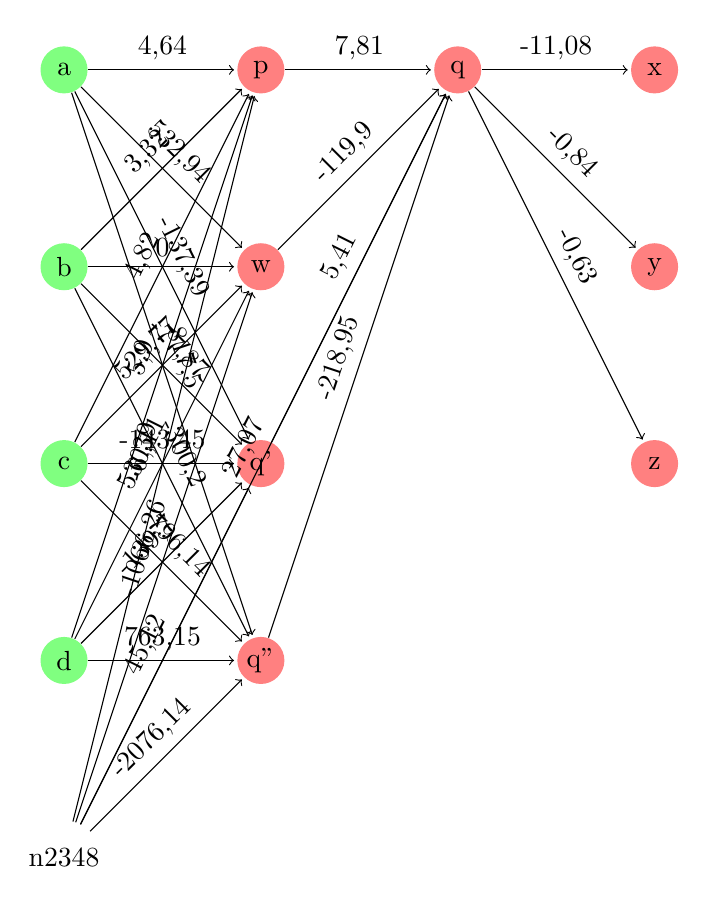
\begin{tikzpicture}[shorten >=1pt,->,draw=black!,node distance=2.5cm]
\tikzstyle{neuron}=[circle,fill=black!25,minimum size=17pt,inner sep=0pt]
\tikzstyle{constant}=[neuron, fill=white!50];
\tikzstyle{sigmoid}=[neuron, fill=red!50];
\tikzstyle{identity}=[neuron, fill=green!50];
\node [identity] (a) {a};
\node [identity,below of=a] (b) {b};
\node [identity,below of=b] (c) {c};
\node [identity,below of=c] (d) {d};
\node [constant,below of=d] (n2348) {n2348};
\node [sigmoid,right of=a] (p) {p};
\node [sigmoid,below of=p] (w) {w};
\node [sigmoid,below of=w] (q') {q'};
\node [sigmoid,below of=q'] (q'') {q''};
\node [sigmoid,right of=p] (q) {q};
\node [sigmoid,right of=q] (x) {x};
\node [sigmoid,below of=x] (y) {y};
\node [sigmoid,below of=y] (z) {z};
\path[every node/.style={sloped,anchor=south,auto=false}]
(q'') edge node {-218,95} (q)
(q') edge node {5,41} (q)
(b) edge node {0} (w)
(b) edge node {3,32} (p)
(b) edge node {-300,2} (q'')
(b) edge node {-77,87} (q')
(a) edge node {4,64} (p)
(a) edge node {-137,39} (q')
(a) edge node {532,94} (w)
(a) edge node {817,5} (q'')
(q) edge node {-0,84} (y)
(q) edge node {-11,08} (x)
(q) edge node {-0,63} (z)
(d) edge node {530,11} (w)
(d) edge node {5,9} (p)
(d) edge node {763,15} (q'')
(d) edge node {-139,7} (q')
(c) edge node {4,82} (p)
(c) edge node {-143,45} (q')
(c) edge node {529,77} (w)
(c) edge node {796,14} (q'')
(n2348) edge node {-6,39} (p)
(n2348) edge node {-1066,26} (w)
(n2348) edge node {27,07} (q)
(n2348) edge node {45,12} (q')
(n2348) edge node {-2076,14} (q'')
(w) edge node {-119,9} (q)
(p) edge node {7,81} (q)
;\end{tikzpicture}
\end{document}